% !TEX program = pdflatex
% !TEX encoding = UTF-8
% !TEX spellcheck = en_US

\documentclass[11pt, a4paper, notitlepage]{article}

\usepackage{settings}

\geometry{margin=1cm}
\graphicspath{./}
\addbibresource[label=main]{./publications.bib}

%--------------------------------------DOCUMENT------------------------------------
\begin{document}
\fontencoding{T1}\selectfont
\pagestyle{empty}
%------------------------------------- ENGLISH VERSION -----------------------------------------------	
	\selectlanguage{english}
		
	\cvname{Milan Skocic, PhD}
	
	\cvjob{Electrochemistry and Materials}
	
	\cvinfo{milan.skocic@icloud.com}
	{+33(0)6 66 18 69}
	{github.com/MilanSkocic}
	{2500C Route de Saint Sernin, 71200 Saint Sernin du Bois, France}
	{0000-0003-2189-5766}
	
	
    %----------------------------------------------------------------------------------------------
	\section*{Work Experience}
		\cventry{May 2017}{Now}{PhD, Electrochemist}{Framatome}{France}
		\begin{jobdetails}
			\item Project Management
			\item High temperature electrochemistry
			\item Corrosion of Zr-based and Ni-based alloys in aqueous high temperature environment
		\end{jobdetails}
		
		\cventry{Oct. 2015}{Feb. 2017}{PhD, Metallic Material}{Areva NP}{France}
		\begin{jobdetails}
			\item Project Management
			\item Stress corrosion cracking in Inconel 718: HT/HP slow tensile tests
			\item Corrosion of Zr-based alloys: HT/HP electrochemistry
		\end{jobdetails}

		\cventry{Oct.2012}{Oct. 2015}{PhD Project - ”Photoelectrochemical study of the Shadow Corrosion”}{Areva/SIMaP Lab}{France}
		\begin{jobdetails}
			\item Design and realization of a new electrochemical cell for HT/HP corrosion tests
			\item Validation of the HT/HP electrochemical cell
			\item HT/ HP (photo-)electrochemical characterizations
			\item Classical corrosion tests in autoclaves at HT and HP
			\item Coupling with chemistry loop
		\end{jobdetails}

		\cventry{Feb. 2012}{Aug. 2012}{Master Intership - ”Metallic bipolar plates for PEMFC”}{Air Liquide}{France}
		\begin{jobdetails}
			\item State of the art of the coated stainless steels
			\item Set-up of the electrochemical tests
			\item Measurement of the interfacial contact resistance
			\item TEM/SEM observations
			\item Go between the different partners involved in the project
		\end{jobdetails}

		\cventry{Apr. 2011}{Aug. 2011}{Master Internship - ”Compositionally graded steels”}{McMaster University, Materials Engineering Department}{Canada}
		\begin{jobdetails}
			\item Carburization of microtruss samples
			\item Prepared and characterized the samples (phase fraction)
			\item Modelling of compressive peak stress
		\end{jobdetails}
		
		\cventry{2007}{2009}{Technician}{ArcelorMittal R\&D center}{France}
		\begin{jobdetails}
			\item Prepared samples: cutting, mounting, polishing
			\item Used microstructural characterization devices: SEM-FEG, TEM, RX diffractometer
			\item Used thermo-mechanical treatment devices: Gleeble, hot rolling pilot, tensile tests
		\end{jobdetails}

		\cventry{Aug. 2005}{Jun. 2006}{Technician}{Pyrolisis Center (CPM)}{France}
		\begin{jobdetails}
			\item Carried out pyrolysis tests on pilot furnace
			\item Prepared and characterized coke and coal samples
		\end{jobdetails}

	\newpage

    %----------------------------------------------------------------------------------------------
    \section*{Education}
	\cvedentry{2012}{2015}{PhD, Materials and Electrochemistry}{University of Grenoble}{France}

	\cvedentry{2012}{2015}{Engineer, Electrochemistry}{Grenoble INP (PHELMA)}{France}
	
	\cvedentry{2003}{2005}{Technician, Analytical Chemistry}{University of Metz}{France}
     
    
    %----------------------------------------------------------------------------------------------
    \section*{Language Skills}
    Serbian \faStar\faStar\faStar\faStar\faStar \hfill
    French \faStar\faStar\faStar\faStar\faStar \hfill
    English \faStar\faStar\faStar\faStar\faStarO

    %----------------------------------------------------------------------------------------------
    \section*{Computer Skills}
    \begin{center}
    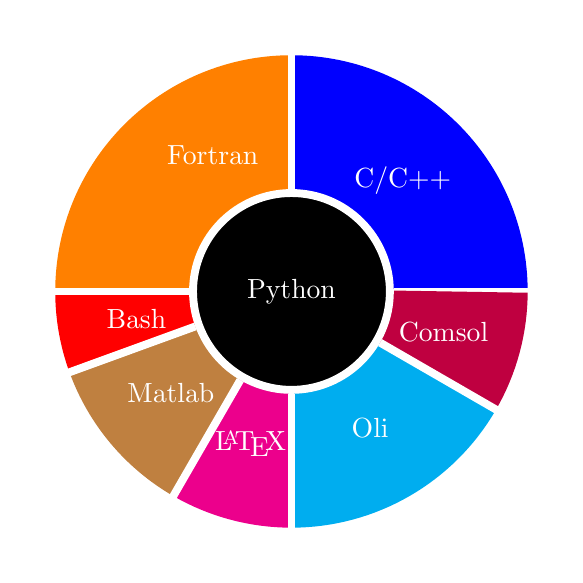
\begin{tikzpicture}[text=white, border/.style={line width=20mm}]
	\foreach \angle/\col [remember=\angle as \last (initially 0)] 
	    in {90/blue, 180/orange, 200/red, 240/brown, 270/magenta, 330/cyan, 360/purple}{
		\draw[\col, border] (\last:2cm) arc[start angle=\last, end angle=\angle, radius=2cm];
		\draw[white, line width=1mm] (\last:1.3)--++(\last:2.0);}
		\node[line width=1mm, draw, circle, minimum width=2.5cm, white, fill=black]{Python};
		\node at (45:2cm) {C/C++};
		\node at (120:2cm) {Fortran};
		\node at (190:2cm) {Bash};
		\node at (220:2cm) {Matlab};
		\node at (255:2cm) {\LaTeX};
		\node at (300:2cm) {Oli};
		\node at (345:2cm) {Comsol};

    \end{tikzpicture}
    \end{center}

    %----------------------------------------------------------------------------------------------
    \section*{PhDs - Technical Mentoring}

    \href{https://tel.archives-ouvertes.fr/tel-02304680/}{S. El Euch, “Recherche d’une corrélation entre caractéristiques électrochimiques et relâchement en nickel de l’alliage 690 en milieu primaire d’un réacteur à eau pressurisée,” Université Sorbonne, Paris, 2019.}
 	
    \href{http://www.theses.fr/s222058}{F. Da Fonseca, “Etude du phénomène de shadow corrosion des alliages de zirconium dans les réacteurs à eau bouillante (REB),” Université de Grenoble Alpes, Grenoble, 2021.}


    \href{http://www.theses.fr/s217506}{J. Ben Mohamed, “Etude des mécanismes de Corrosion sous contrainte des alliages 600/690 en milieu secondaire des réacteurs REP en présence de plomb et de soufre.,” Ecole Nationale Supérieure des Mines de Saint-Etienne, Saint-Etienne, 2021.}
    
    \href{http://www.theses.fr/s278984}{D. Peyret, “Mécanismes électrochimiques de la corrosion des alliages de type ZrNbX en condition simulées de réacteur à eau pressurisée,” Université Sorbonne, Paris, 2023.}
	

    %----------------------------------------------------------------------------------------------
    \newpage
	\nocite{*}
	\printbibliography[title=Publications]
	
\end{document}
